\documentclass{article}


\usepackage{../../austin137}
\usepackage{../../local}
\usehyperstuff
\usepackage{wrapfig}

\begin{document}

%%%%%%%%%%%%%%%%%%%%%%%%%%%%%%%%%%%%%%%%%%%%%%%%%%%%%%%%%%%%%%%%%%%%%%%%%%%%%%%%
\addcopyright
\begin{center}
{\bf \large Physics W89 - Introduction to Mathematical Physics - Summer 2023}\\\medskip
{\bf \large Problem Set - Module 03 - The Matrix} \\\medskip
{\emph{Last Update: \today}\\}
{Student: Yutong (Eric) Du}
\end{center}


\dphline\bigskip
%%%%%%%%%%%%%%%%%%%%%%%%%%%%%%%%%%%%%%%%%%%%%%%%%%%%%%%%%%%%%%%%%%%%%%%%%%%%%%%%
\section*{Problem 3.1 - Rotations}
\relevid{Introduction to Matrices; Matrix Multiplication}

%%%%%%%%%%%%%%%%%%%%%
\paragraph{}
In this problem we will look at an important set of linear transformations in physics, \heavydef{rotations}.
First, let's just consider rotations in the plane ($\mathbb{R}^{2}$).  You can picture the vector space $\mathbb{R}^{2}$ as the space of ``arrows in the plane'' 
as discussed in lecture.  Let $\{\hat{x},\hat{y}\}$ be an orthonormal basis for this space, with $\hat{x}$ being the ``to the right of the page'' direction and $\hat{y}$ being the 
``to the top of the page'' direction.  Let $\mathsf{R}_{\theta}$ be the transformation that rotates a vector counterclockwise in the plane by an angle of $\theta$.  Since
$\mathsf{R}_{\theta}$ takes an arrow in the plane and returns another arrow in the plane, we write $\mathsf{R}_{\theta}: \mathbb{R}^{2} \to \mathbb{R}^{2}$.  
Vectors in the plane can be represented as $(2\times 1)$ column vectors and the rotation can be represented as a $(2\times 2)$ matrix.


%%%%%%%%%%%%%%%%%%%%%
\paragraph{(a)}
Using geometry and trigonometry (that is, pictures and diagrams and such, without need of our fancy new matrix language), determine how $\hat{x}$ and $\hat{y}$ 
transform under this rotation.  Use this result to write down the matrix for the transformation $\mathsf{R}_{\theta}$.

\begin{solution}
	Consider the following diagram showing a vector $\vec v'$ that's gone under a rotation $\theta$:
	
	\begin{center}
		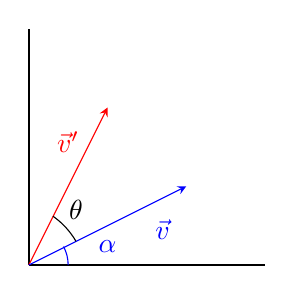
\begin{tikzpicture}
			\draw[thick] (0, 0) -- (3, 0);
			\draw[thick] (0, 0) -- (0, 3);
			\draw[-stealth, red] ( 0, 0) -- (1, 2);
			\draw[red] (0.5, 1.3) node[above] {$\vec v'$}; 
			\draw[-stealth, blue] (0, 0) -- (2, 1); 
			\draw[blue] (1.7, 0.7) node[below] {$\vec v$};
			\draw (0.6, 0.3) arc(30:55:1) ; 
			\draw (0.6, 0.45) node[above] {$\theta$};
			\draw[blue] (0.5, 0) arc(0:28:0.5);
			\draw[blue] (1, 0.03) node[above] {$\alpha$};
		\end{tikzpicture}
	\end{center}

		Initially, we can represent the location of the vector $\vec v$ as:
		\[
		\vec v = \begin{pmatrix} |\vec v| \cos \alpha\\ |\vec v| \sin \alpha \end{pmatrix} 
		\] 
		Now, we can represent the location of the vector $\vec v'$ as:
		\[
		\vec v' = \begin{pmatrix} |\vec v| \cos (\alpha + \theta)\\
		|\vec v| \sin(\alpha + \theta) \end{pmatrix} 
		\] 
		Then, we want to use the rotation matrix and link these two together. The rotation operation, written as
		a matrix multiplication, can be represented as:
		\[
			\begin{pmatrix} R_{11} & R_{12}\\R_{21} & R_{22} \end{pmatrix} \begin{pmatrix} |\vec v| \cos \alpha\\
			|\vec v| \sin \alpha \end{pmatrix} = \begin{pmatrix} |\vec v| \cos(\alpha + \theta)\\
		|\vec v| \sin(\alpha + \theta) \end{pmatrix} 
		\] 
		Now we can use trigonometric identities to simplify the right hand side, while doing standard matrix 
		multiplication on the left hand side:
		\[
		\begin{pmatrix} R_{11}|\vec v| \cos \alpha + R_{12}|\vec v| \sin \alpha \\
			R_{21}|\vec v| \cos \alpha + R_{22}|\vec v| \sin \alpha \end{pmatrix}  =
			\begin{pmatrix} |\vec v|(\cos \alpha \cos \theta - \sin \alpha \sin \theta)\\ 
			|\vec v|(\sin \alpha \cos \theta + \cos \alpha \sin \theta)  \end{pmatrix} 
		\] 
		Then comparing the terms, we find that:
		\begin{align*}
			R_{11} &= \cos \theta\\
			R_{12} &= -\sin \theta \\
			R_{21} &=  \sin \theta \\
			R_{22} &=  \cos \theta 
		\end{align*}
		Thus, the rotation matrix is:
		\[
			R = \begin{pmatrix} \cos \theta & -\sin \theta \\ \sin \theta & \cos \theta \end{pmatrix} 
		\] 
		the beginning of part (b) also confirms this result. 
\end{solution}

%%%%%%%%%%%%%%%%%%%%%
\paragraph{(b)}
You should have found the matrix $\mathsf{R}_{\theta}\doteq \smmatrix{0.8}{\cos\theta&-\sin\theta\\\sin\theta&\cos\theta}$ in part (a).\footnote{Spoilers!}
	\begin{itemize}
		\item Find all the vectors in $\mathbb{R}^{2}$ that are left unchanged by $\mathsf{R}_{\theta}$. (For $0<\theta<2\pi$.  If $\theta=0$ then the rotation
		matrix becomes the identity matrix and \emph{all} vectors in $\mathbb{R}^{2}$ are left unchanged!)

			\begin{solution}
				Since the rotation will change any nonzero vector, only the zero vector $\vec 0$ remains 
				unchanged after a rotation by an angle $\theta$.
			\end{solution}
		\item Show that acting $\mathsf{R}_{\theta}$ on a vector leaves the magnitude of the vector unchanged.

			\begin{solution}
				Computing the magnitude of $v'$:
				\begin{align*}
					|v'| &= \sqrt{(|\vec v|^2 \cos^2(\alpha + \theta) + |\vec v|^2 \sin^2(\alpha + \theta)} \\
					&= \sqrt{|\vec v|^2(1)}  \\
					&= |\vec v| 
				\end{align*}
			\end{solution}
		\item More generally, show that the dot product of two vectors $\vec{v}\cdot\vec{w}$ is the same as the dot product of the rotated vectors 
		$(\mathsf{R}_{\theta}\vec{v})\cdot(\mathsf{R}_{\theta}\vec{w})$.

		\begin{solution}
			Dotting $\vec v \cdot \vec w$:
			\[
				\vec v \cdot \vec w = \begin{pmatrix} |\vec v| \cos \alpha_1 & |\vec v| \sin \alpha_1 
				\end{pmatrix} \begin{pmatrix} |\vec w| \cos \alpha_2 \\ |\vec w| \sin \alpha_2 \end{pmatrix} 
			\] 
			Note we can do this without taking the complex conjugate since we're working in $\mathbb R^2$, which 
			means we're only dealing with real vectors. Anyways, the dot product becomes: 
			\[
			\vec v \cdot \vec w = |\vec v| |\vec w| \cos (\alpha_1 - \alpha_2)
			\] 
			Now if we take the rotated vectors, we know that they can be represented as (from part (a)): 
			\begin{align*}
				R_{\theta} \vec v &= \begin{pmatrix} |\vec v| \cos(\alpha_1 + \theta) \\
				|\vec v| \sin(\alpha_1 + \theta)  \end{pmatrix} \\
					R_{\theta} \vec w &= \begin{pmatrix} |\vec w| \cos(\alpha_2 + \theta) \\ |\vec w| \sin (\alpha_2 + \theta)  \end{pmatrix} 
			\end{align*}
			Then if we dot these two vectors, we get: 
			\begin{align*}
				(R_\theta \vec v) \cdot (R_\theta \vec w) &=
				\begin{pmatrix} |\vec v| \cos(\alpha_1 + \theta) & |\vec v| \sin(\alpha_1 + \theta) \end{pmatrix}
				\begin{pmatrix} |\vec w| \cos(\alpha_2 + \theta) \\ |\vec w| \sin(\alpha_2 + \theta)  
				\end{pmatrix} \\
				&= |\vec v| |\vec w| \cos(\alpha_1 + \theta) \cos(\alpha_2 + \theta) + 
				|\vec v| |\vec w|\sin(\alpha_1 + \theta) \sin(\alpha_2 + \theta)   \\
				&= |\vec v| |\vec w| \cos\left[(\alpha_1 + \theta) - (\alpha_2 + \theta)\right] \\
				&= |\vec v| |\vec w| \cos(\alpha_1 - \alpha_2) 
			\end{align*} 
			which is exactly the result we got from dotting the two original vectors $\vec v \cdot \vec w$. 
			Thus, we come to the conclusion that 
			\[
			\vec v \cdot \vec w = (R_\theta \vec v) \cdot (R_\theta \vec w)
			\] 
			as desired. 
		\end{solution}
	\end{itemize}
\note{This last property is a result of a matrix property known as \heavydef{orthogonality}.}


%%%%%%%%%%%%%%%%%%%%%
\paragraph{(c)}
Using matrix multiplication, show that first rotating by $\theta_{1}$ and then rotating by $\theta_{2}$ gives the same transformation as rotating by $\theta_{1}+\theta_{2}$.
\spoilers{You will have to use some trigonometric identities here!}

\begin{solution}
	The goal of this part is to show that $R_{\theta_2} R_{\theta_1} \vec v = R_{\theta_1 + \theta_2} \vec v$. 
	So really, we can actually just forget $\vec v$ and instead show that $R_{\theta_2}R_{\theta_1} = R_{\theta_1
	+ \theta_2}$, since if the two transformations are equivalent then acting both on $\vec v$ should produce
	the same result. Now let's multiply $R_{\theta_1} R_{\theta_1}$:
	\begin{align*}
		R_{\theta_2}R_{\theta_1} &= \begin{pmatrix} \cos \theta_2 & - \sin \theta_2\\ \sin \theta_2 & \cos \theta_2 \end{pmatrix} \begin{pmatrix} \cos \theta_1 & - \sin \theta_1\\ \sin \theta_1 & \cos \theta 1 \end{pmatrix} \\
								 &= \begin{pmatrix} \cos \theta_1 \cos \theta_2 - \sin \theta_1 \sin \theta_2 & -\cos \theta_2 \sin \theta_1 - \sin \theta_2 \cos \theta_1\\ \sin \theta_2 \cos \theta_1 + \cos \theta_2 \sin \theta_1 & -\sin \theta_2 \sin \theta_1 + \cos \theta_2 \cos \theta_1 \end{pmatrix} 
	\end{align*}
	Now we remember our identities: 
	\begin{align*}
		\cos (\theta_1 + \theta_2) = \cos \theta_1 \cos \theta_2 - \sin \theta_1 \sin \theta_2\\
		\sin(\theta_1 + \theta_2) = \sin \theta_1 \cos \theta_2 + \cos\theta_1 \sin \theta_2
	\end{align*}
	Now we see that all four entries of our matrix actually correspond to one of these identities. Specifically: 
	\[
		\begin{pmatrix} \cos \theta_1 \cos \theta_2 - \sin \theta_1 \sin \theta_2 & -\cos \theta_2 \sin \theta_1 - \sin \theta_2 \cos \theta_1\\ \sin \theta_2 \cos \theta_1 + \cos \theta_2 \sin \theta_1 & -\sin \theta_2 \sin \theta_1 + \cos \theta_2 \cos \theta_1 \end{pmatrix} = \begin{pmatrix} \cos(\theta_1 + \theta_2) & -\sin (\theta_1 + \theta_2) \\ \sin(\theta_1 + \theta_2) & \cos(\theta_1 + \theta_2) \end{pmatrix} 
	\] 
	Now notice that this resulting matrix is just the rotation matrix, except now with the angle 
	$\theta_1 + \theta_2$ as the angle we are rotating by. This was exactly what we needed to show: that 
	first rotating by $\theta_1$ then by $\theta_2$ (represented by the matrix multiplication) is equivalent
	to rotating by a total angle of $\theta_1 + \theta_2$. 
\end{solution}


%%%%%%%%%%%%%%%%%%%%%
\paragraph{}
Lets move to three dimensions!  Let $\mathsf{R}(\hat{n},\theta)$ be a right-handed rotation by angle $\theta$ about the axis $\hat{n}$.\footnote{By ``right-handed,''
we mean: point the thumb of your right hand in the direction of the axis $\hat{n}$.  Your finger then curl around your thumb in the direction of the rotation.}  The rotation
matrices about the three axes $\hat{x}$, $\hat{y}$, and $\hat{z}$ in three dimensions are
	\begin{equation*}
		\mathsf{R}(\hat{x},\theta) = \smmatrix{0.9}{1 & 0 & 0 \\ 0 & \cos\theta & -\sin\theta \\ 0 & \sin\theta & \cos\theta},	\qquad
		\mathsf{R}(\hat{y},\theta) = \smmatrix{0.9}{\cos\theta & 0 & \sin\theta \\ 0 & 1 & 0 \\ -\sin\theta & 0 & \cos\theta}, \qquad
		\mathsf{R}(\hat{z},\theta) = \smmatrix{0.9}{\cos\theta & -\sin\theta & 0 \\ \sin\theta & \cos\theta & 0 \\ 0 & 0 & 1}.
	\end{equation*}


\paragraph{(d)}
Check that $\mathsf{R}(\hat{x},\pi/2)$, $\mathsf{R}(\hat{y},\pi/2)$, and $\mathsf{R}(\hat{z},\pi/2)$ all give the expected result when acting on the vector $\hat{x}$.\\
\note{First consider a set of coordinate axes: $\hat{x}$ to the right of the page, $\hat{y}$ to the top of the page, and $\hat{z}$ coming out of the plane of the page - and
determine what a right-handed rotation by 90 degrees does to the vector $\hat{x}$.  Then see what the matrices $\mathsf{R}$ do to $\hat{x} \doteq \smthreevect{1}{0}{0}$
and see if they agree!}


	\begin{solution}
		First, let's just think about what should happen. For $R_x \hat{x}$, we should expect that this 
		transformation leaves $\hat{x}$ untouched, since a rotation of $\hat{x}$ about its own axis does 
		not rotate the vector at all. 

		For $R_y \hat{x}$, we should expect that a right-handed rotation sends $\hat{x}$ to $-\hat{z}$, if
		we follow through with right hand rule and rotating by $90^\circ$. 

		For $R_z \hat{x}$, we should expect that a right-handed rotation sends $\hat{x}$ to $\hat{y}$, again 
		just following through with the right hand rule and rotating by $90^\circ$. 

		Now, let's plug  $\theta = \frac{\pi}{2}$ into all three of these matrices, we get:
		\begin{align*}
			R_x &= \begin{pmatrix} 1&0&0\\0&0&-1\\0&1&0 \end{pmatrix} \\
			R_y &=  \begin{pmatrix} 0&0&1\\0&1&0\\-1&0&0 \end{pmatrix}  \\
			R_z &= \begin{pmatrix} 0&-1&0\\1&0&0\\0&0&1 \end{pmatrix} 
		\end{align*}
		Performing these operations on $\hat{x} = \smthreevect{1}{0}{0}$ gives:
		\begin{align*}
			R_x \hat{x} &= \begin{pmatrix} 1&0&0\\0&0&-1\\0&1&0 \end{pmatrix}\begin{pmatrix} 1\\0\\0 \end{pmatrix} = \begin{pmatrix} 1\\0\\0 \end{pmatrix} \\
			R_y \hat{x} &= \begin{pmatrix} 0&0&1\\0&1&0\\-1&0&0 \end{pmatrix} \begin{pmatrix} 1\\0\\0 \end{pmatrix}	= \begin{pmatrix} 0\\0\\-1 \end{pmatrix} \\
			R_z \hat{x} &=  \begin{pmatrix} 0&-1&0\\1&0&0\\0&0&1 \end{pmatrix} \begin{pmatrix} 1\\0\\0 \end{pmatrix} = \begin{pmatrix} 0\\1\\0 \end{pmatrix} 
\\
		\end{align*}
		These three results match exactly what we expected from the beginning: $R_x$ leaves $\hat{x}$ unchanged,
		$R_y$ sends $\hat{x}$ to $-\hat{z}$, and $R_z$ sends $\hat{x}$ to $\hat{y}$. 
	\end{solution}

%%%%%%%%%%%%%%%%%%%%%
\paragraph{}
The rotation matrices can actually be written as the \emph{exponentials} of other matrices.  For example, a counterclockwise rotation in a 2D plane can be written
	\begin{equation}
		\mathsf{R}_{2D}(\theta) = e^{\theta \mathsf{L}}, \qquad \mbox{where} \quad 	\mathsf{L} = \smmatrix{0.9}{0 & -1 \\ 1 & 0}.
	\label{RotationExp}
	\end{equation}
But... but... how can we exponentiate a \emph{matrix}!?  The same way we learned how to exponentiate a complex number - by using the Taylor expansion.  If
$\mathsf{M}$ is a square matrix (having the same number of rows and columns), then we define $\mathsf{M}^{0}$ to be the identity matrix (with 1 for all the diagonal elements, 
and 0 for all other elements) and define the \heavydef{matrix exponential} to be
	\begin{equation*}
		e^{\mathsf{M}} \equiv \sum_{n=0}^{\infty} \frac{\mathsf{M}^{n}}{n!}.
	\end{equation*}


\paragraph{(e)}
To perform the exponential in Eq.~\ref{RotationExp} first we need to find $\mathsf{L}^{n}$.  Write down $\mathsf{L}^{0}$ and $\mathsf{L}^{1}$ (these require no work).  Then
explicitly use matrix multiplication to find $\mathsf{L}^{2}$, $\mathsf{L}^{3}$, and $\mathsf{L}^{4}$.  Try to guess the pattern that occurs after this. (Answer provided below!)

\begin{solution}
	$L^0$ is the identity by the given definition, and $L^1$ is just the matrix $L$ istelf, so therefore: 
	\begin{align*}
		L^0 &= \begin{pmatrix} 1&0\\0&1 \end{pmatrix}  \\
		L^1 &= \begin{pmatrix} 0&-1\\1&0 \end{pmatrix} 
	\end{align*}
	Now we have to use matrix multiplication to find $L^2$ and the other powers: 
	\begin{align*}
		L^2 &= \begin{pmatrix} 0 & -1 \\ 1 & 0 \end{pmatrix} \begin{pmatrix} 0 & -1 \\1&0 \end{pmatrix} = \begin{pmatrix} -1 & 0 \\ 0 & -1 \end{pmatrix} \\
		L^3 &= \begin{pmatrix} -1 & 0 \\0 & -1 \end{pmatrix} \begin{pmatrix} 0 &-1 \\1 & 0 \end{pmatrix} = \begin{pmatrix} 0 & 1\\-1 & 0 \end{pmatrix}  \\
		L^4 &= \begin{pmatrix} 0 & 1\\-1&0 \end{pmatrix} \begin{pmatrix} 0 & -1 \\ 1 & 0 \end{pmatrix} = \begin{pmatrix} 1 & 0\\0&1 \end{pmatrix} 
	\end{align*}
	Here, we notice a couple things: firstly, $L^4$ is the identity matrix. This makes sense, since rotating 
	something $90^\circ$ 4 times is rotating a full circle, so we should get the same matrix back. Further, we 
	also find that $L^3 = -L^1$, and $L^2 = -L^0$. This suggests some sort of alternating pattern.
\end{solution}
%%%%%%%%%%%%%%%%%%%%%
\paragraph{}
The $n$-th power of $\mathsf{L}$ for $n=1,2,3,\cdots$ winds up being
	\begin{equation*}
		\mathsf{L}^{n} = \begin{cases}
			(-1)^{(n-1)/2}\mathsf{L},	& \mbox{$n$ odd},\\
			-(-1)^{n/2}\mathsf{L}^{2},	& \mbox{$n$ even}
		\end{cases}.
	\end{equation*}


\paragraph{(f)}
Use the above results and the known Taylor series for $e^{x}$, $\cos x$, and $\sin x$ to find the matrix for the rotation $\mathsf{R}_{2D}(\theta) = e^{\theta \mathsf{L}}$.

\begin{solution}
	We use the definition of the taylor expansion:
	\[
		e^{\theta L} = \sum_{n=0}^\infty \frac{(\theta L)^n}{n!} = \frac{\theta^0 L^0}{0!} + \frac{\theta^1 L^1}{1!} + \frac{\theta^2L^2}{2!} + \dots
	\] 
	Expanding this out in terms of what we have for the powers of $L$, we get:
	\begin{align*}
		e^{\theta L} &= \begin{pmatrix} 1 & 0\\0&1 \end{pmatrix} + 
		\begin{pmatrix} 0 & -\theta \\ \theta & 0 \end{pmatrix} +
		\begin{pmatrix} -\theta^2 / 2 & 0 \\ 0 & -\theta ^2/2 \end{pmatrix} +
		\begin{pmatrix} 0 & \theta^3 /6\\ - \theta^3 /6 & 0 \end{pmatrix} + \dots\\
						  &= \begin{pmatrix} 1 - \frac{\theta^2}{2} + \frac{\theta^4}{24} + \dots & -\left[\theta - \frac{\theta^3}{6} + \dots \right]\\ \theta - \frac{\theta^3}{6} + \dots & 1 - \frac{\theta^2}{2} + \frac{\theta^4}{24} + \dots \end{pmatrix} 
	\end{align*} 
	what we notice is that each element of the matrix actually represents the Taylor series for one of $\cos x$
	or $\sin x$. Specifically, we know that: 
	\begin{align*}
		\sin \theta &= \theta - \frac{\theta^3}{3!} + \dots = \theta - \frac{\theta^3}{6} + \dots\\
		\cos \theta &= 1 - \frac{\theta^2}{2} + \frac{\theta^4}{4!} + \dots = 1 - \frac{\theta^2}{2} + \frac{\theta^4}{24} + \dots
	\end{align*} 
	so therefore if we look back at our matrix, we find that this matrix can actually be written as:
	\[
		\begin{pmatrix} 1 - \frac{\theta^2}{2} + \frac{\theta^4}{24} + \dots & -\left[\theta - \frac{\theta^3}{6} + \dots \right]\\ \theta - \frac{\theta^3}{6} + \dots & 1 - \frac{\theta^2}{2} + \frac{\theta^4}{24} + \dots \end{pmatrix} = \begin{pmatrix} \cos \theta & - \sin \theta\\ \sin \theta & \cos \theta   \end{pmatrix} 
	\] 
	which matches exactly what we had before as the rotation matrix in 2D. 
\end{solution}

\bigskip
\pagebreak
%%%%%%%%%%%%%%%%%%%%%%%%%%%%%%%%%%%%%%%%%%%%%%%%%%%%%%%%%%%%%%%%%%%%%%%%%%%%%%%%
\section*{Problem 3.2 - Solving a DC Circuit}
\relevid{Linear Systems of Equations as Matrix Equations; Gauss-Jordan Reduction (Row Reduction); Linear Independence \& Existence and Uniqueness of Solutions}

%%%%%%%%%%%%%%%%%%%%%
\paragraph{}
\begingroup\setlength\intextsep{-5pt}
	%~~~~~~~~~~~~~~ FIGURE ~~~~~~~~~~~~~~%
	\begin{wrapfigure}[6]{r}{0cm}
		\includegraphics[width = 0.35\textwidth]{89-PS3-P2-Circuit}
	\end{wrapfigure}
	%~~~~~~~~~~~~~~ FIGURE ~~~~~~~~~~~~~~%
The figure to the right shows a DC circuit consisting of a battery of voltage $\EMF$ and a resistor of resistance $R$ on the left branch, a battery of voltage $2\EMF$
and a resistor of resistance $2R$ on the middle branch, and a resistor with resistance $6R$ on the right branch.  We can determine the unknown currents $I_{1}$,
$I_{2}$, and $I_{3}$ by using the Kirchhoff circuit rules to create a system of linear equations.


%%%%%%%%%%%%%%%%%%%%%
\paragraph{(a)}		\extrapart
Time to apply your second semester physics knowledge!\footnote{Only taking second-semester physics now?  Don't worry!  That's why this is a not-for-credit part.  You can use
this problem when you get to the DC circuits unit as extra practice!}  Identify two junctions and three loops for this circuit and write down the associated junction and loop
rules to create a system of five linear equations in three unknowns.
\endgroup

\phline
%%%%%%%%%%%%%%%%%%%%%
\paragraph{}
One possible system of equations you can get by applying Kirchhoff's laws for this circuit is given by
	\begin{alignat*}{2}
		\mbox{Top Junction:}&\qquad& I_{1}+I_{2}-I_{3} &=0,\\
		\mbox{Bottom Junction:}&\qquad& I_{3}-I_{1}-I_{2} &=0,\\
		\mbox{Left Loop:}&\qquad& \EMF - I_{1}R + 2I_{2}R - 2\EMF &=0,\\
		\mbox{Right Loop:}&\qquad& 2\EMF - 2I_{2}R - 6I_{3}R &=0,\\
		\mbox{Outer Loop:}&\qquad& \EMF - I_{1}R - 6I_{3}R &=0.
	\end{alignat*}
If we let $\vec{x} \equiv \smthreevect{I_{1}}{I_{2}}{I_{3}}$ be the vector of three unknown currents we can rewrite the above system of equations as a matrix equation 
$\mathsf{A}\vec{x}=\vec{b}$, where $\mathsf{A}$ is an $(m\times n)$-matrix.


\paragraph{(b)}
What are $m$ and $n$ for the matrix $\mathsf{A}$?  How many entries does $\vec{b}$ have?  Do a quick sanity check to see that this matrix
multiplication works out properly (that is, the number of rows and columns in $\mathsf{A}$ and $\vec{x}$ are consistent with a matrix multiplication to get
the vector $\vec{b}$).  Find the matrix of coefficients $\mathsf{A}$ and the column vector of constants $\vec{b}$ for the above system of equations.


\begin{solution}
	The matrix $A$ can be written as: 
	\[
		A = \begin{pmatrix} 1 & 1 & -1\\ -1 &-1 & 1\\ -R & 2R & 0 \\ 0 & -2R & -6R\\ -R & 0 & -6R \end{pmatrix} 
	\] 
	There are 5 rows and 3 columns, meaning we have a $5 \times 3$ matrix, hence $m = 5$ and $n = 3$. The vector
	$\vec b$ can be written as: 
	\[
	\vec b = \begin{pmatrix} 0 \\ 0 \\ \mathcal E \\ -2 \mathcal E\\-\mathcal E \end{pmatrix} = \mathcal E
	\begin{pmatrix} 0 \\ 0 \\ 1 \\ -2 \\ -1  \end{pmatrix} 
	\] 
	This is a $5 \times 1$ matrix. We can then verify that from matrix multiplication, multiplying a $5\times 3$
	matrix by a $3 \times 1$ matrix (which is $\vec x$) indeed generates a $5 \times 1$ matrix, meaning that 
	the matrix multiplication is consistent.
	
\end{solution}

%%%%%%%%%%%%%%%%%%%%%
\paragraph{(c)}
Write down the augmented matrix $\tilde{\mathsf{A}}$ and perform a Gauss-Jordan reduction to reduce it to reduced row echelon form. Underline the ``pivotal 1''s in your
reduced matrix.

\begin{solution}
	Now we begin the painful process of row reduction. Starting off, we write the augmented matrix: 
	\[
		\tilde A = \begin{pmatrix} 1 &1 & -1 & 0\\ -1 & -1 & 1 & 0\\ -R & 2R & 0 & \mathcal E \\ 
		0 & -2R & -6R & -2\mathcal E\\ -R & 0 & -6R & -\mathcal E \end{pmatrix} 
	\] 
	First, we can add row 1 to row 2, and also simultaneously subtract row 3 from row 5:
	\[
		\tilde A = \begin{pmatrix} 1 & 1 & -1 & 0 \\ 0&0&0&0\\-R&2R&0&\mathcal E\\0&-2R&-6R &-2\mathcal E\\
		0&-2R&-6R&-2\mathcal E\end{pmatrix} 
	\] 
	Then we subtract row 4 from row 5, then divide row 4 by 2. At this point, we have two rows full of zeroes, 
	so we can put these two rows at the bottom of the matrix: 
	\[
		\begin{pmatrix} 1 & 1 & -1 &0\\-R&2R&0&\mathcal E\\0&-R&-3R&-\mathcal E\\0&0&0&0\\0&0&0&0 \end{pmatrix} 
	\] 
	Then we add $R$ times row 1 to row 2:
	\[
		\begin{pmatrix} 1 & 1& -1 &0\\0 & 3R & -R & \mathcal E\\0 & -R & -3R & -\mathcal E\\ 0&0&0&0\\0&0&0&0
		\end{pmatrix} 
	\] 
	For simplicity we will multiply row 1 by $R$, then add 3 times row 3 to row 2:
	\[
		\begin{pmatrix} R & R &-R&0\\0&0&-10R&-2\mathcal E\\0 &-R&-3R&-\mathcal E\\0&0&0&0\\0&0&0&0
		\end{pmatrix} 
	\] 
	Now add row 3 to row 1 and after doing so swap rows 2 and 3:
	\[
		\begin{pmatrix} R&0&-4R &-\mathcal E\\0&0&-5R &-\mathcal E\\0&-R&-3R&-\mathcal E\\0&0&0&0\\0&0&0&0
			\end{pmatrix} = \begin{pmatrix} R&0&-4R&-\mathcal E\\0&-R&-3R&-\mathcal E\\0&0&-5R&-\mathcal E \\0&0&0&0\\0&0&0&0
	\end{pmatrix} 
	\] 
	Now multiply row 3 by $-4 / 5$ then add this to row 1, and also mutliply row 3 by $-3 / 5$ and add that 
	to row 2. Doing so, we get: 
	\[
		\begin{pmatrix} R &0&0&-\mathcal E/ 5\\0 &-R&0&-2\mathcal E / 5\\ 0&0&-5R & - \mathcal E\\0&0&0&0\\0&0&0&0\end{pmatrix} 
	\] 
	Then divide the first three rows to get the pivotal 1's: 
	\[
		\begin{pmatrix} \underline 1 &0&0&-\mathcal E / 5R\\0 & \underline 1 & 0 & 2\mathcal E / 5R\\ 
		0 &0 & \underline 1 & \mathcal E / 5R\\0&0&0&0\\0&0&0&0 \end{pmatrix} 
	\] 


\end{solution}


%%%%%%%%%%%%%%%%%%%%%
\paragraph{(d)}
Determine the ranks of $\mathsf{A}$ and $\tilde{\mathsf{A}}$.  Will the system of equations have no solutions, a unique solutions, or an infinite number of solutions?
If there is a unique solution, determine the solution!  If there are an infinite number of solutions, determine \emph{one} solution and the dimension of the solution set.

\begin{solution}
	The number of pivotal ones in $A$ is 3, and simultaneously the number of pivotal ones in $\tilde A$ is also
	3. The number of columns of $A$ is also 3, meaning that we have a unique solution. That solution can 
	simply be read off of the matrix: 
	\begin{align*}
		I_1 &= -\frac{\mathcal E}{5R}\\
		I_2 &= \frac{2\mathcal E}{5R} \\
		I_3 &= \frac{\mathcal E}{5R}
	\end{align*}
\end{solution}
%%%%%%%%%%%%%%%%%%%%%
\paragraph{}
For this system we should find that $\rank{\mathsf{A}}$ is two less than the number of rows of $\mathsf{A}$.  We can interpret this as saying we have
two redundant equations.


\paragraph{(e)}		\extrapart
Show explicitly that we can choose two of the original five equations and write them as linear combinations of the other three.


\bigskip
\pagebreak
%%%%%%%%%%%%%%%%%%%%%%%%%%%%%%%%%%%%%%%%%%%%%%%%%%%%%%%%%%%%%%%%%%%%%%%%%%%%%%%%
\section*{Problem 3.3 - Images and Kernels}
\relevid{Linear Independence \& Existence and Uniqueness of Solutions;  Images and Kernels;  Ranks and Nullities}


%%%%%%%%%%%%%%%%%%%%%
\paragraph{}
Consider a linear transformation $\mathsf{M}:V\to W$.  
The \heavydef{image} of $\mathsf{M}$ is the set of all vectors $\vec{w}\in W$ such that $\vec{w}$ can be written as $\mathsf{M}$ acting 
on some vector in $V$.  
The \heavydef{kernel} is the set of all vectors $\vec{v}\in V$ such that $\mathsf{M}$ acting on $\vec{v}$ gives the zero vector $\vec{0}$,
	\begin{align*}
		\Im{\mathsf{M}} &\equiv \{\vec{w}\in W|\,\vec{w} = \mathsf{M}\vec{v}\},\\
		\ker \mathsf{M} &\equiv \{\vec{v}\in V|\,\mathsf{M}\vec{v} = \vec{0}\}.
	\end{align*}

\paragraph{(a)}
Prove that $\Im\,M$ and $\ker\,M$ are vector subspaces of $W$ and $V$, respectively.  \\
\note{We already did this in lecture, but be sure you understand the steps necessary!}

\begin{solution}
	We show first that the image is a vector subspace, starting with addition. Let
	$\vec w_1, \vec w_2 \in W$ where $\vec w_1 = M \vec v_1, \vec w_2 = M\vec v_2$. Then, adding these 
	two vectors: 
	\[
	\vec w_1 + \vec w_2 = M\vec v_1 + M \vec v_2
	\] 
	then abusing the linearity of $M$, we then conclude:
	\[
	M \vec v_1 + M \vec v_2 = M(\vec v_1 + \vec v_2) 
	\] 
	Now, since $V$ is a vector space then $\vec v_1 + \vec v_2 \in V$ and hence $M(\vec v_1 + \vec v_2) \in W$, 
	thus proving that the image is closed under vector addition. Now for scalar multiplication. Let $\vec w 
	\in W$ where $\vec w = M\vec v$ then:
	\[
	c\vec w = c(M\vec v) 
	\] 
	Then by linearity of $M$, we get: 
	\[
	c(M \vec v) = M(c \vec v)
	\] 
	Again, since $c\vec v \in V$ (as $V$ is a vector space), then $M(c \vec V) \in W$, and hence the image is closed under scalar 
	multiplication as well. Since it is closed under both vector addition and scalar multiplication, then 
	the image is a vector subspace of $V$.

	As for the kernel, we can do the same, starting with addition. Here, let $v_1, v_2 \in V$ where $M\vec v_1
	= \vec 0$ and $M \vec v_2 = \vec 0$ (in other words, $v_1, v_2 \in \ker(V)$). Then by linearity in $M$:
	\[
	M(\vec v_1 + \vec v_2) = M\vec v_1 + M\vec v_2 = \vec 0 + \vec 0 = \vec 0
	\] 
	Therefore $\vec v_1+ \vec v_2 \in \ker(M)$, so the kernel is closed under vector addition. For multiplication, again let $\vec v_1 \in \ker(V)$. Again
	using the property that $M$ is linear:
	\[
	M(c \vec v_1) = c(M\vec v_1) = c \vec 0 = \vec 0 \implies c\vec v_1 \in \ker(M)
	\] 
	hence the kernel is also closed under scalar multiplication. Since it is closed under both vector addition 
	and scalar multiplication, the kernel is also a vector subspace of $V$.  
\end{solution}

%%%%%%%%%%%%%%%%%%%%%
\paragraph{}
The \heavydef{column space} of $\mathsf{M}$ is defined as the span of the column vectors that make up the matrix $\mathsf{M}$.  This next part is a nice little proof that the column 
space is equivalent to the image of $\mathsf{M}$!  To prove two spaces $A$ and $B$ are equal we have to show that 
$A\subset B$ and $B \subset A$.  Let $\mathsf{M} = \begin{pmatrix} \vec{\mu}_{1} & \cdots & \vec{\mu}_{m}\end{pmatrix}$, where $\vec{\mu}_{i}$ is the $i$-th column of $\mathsf{M}$.

\paragraph{(b)}
Prove $\Im\mathsf{M}\subset\Span(\vec{\mu}_{1},\cdots, \vec{\mu}_{m})$ by showing that $\mathsf{M}\vec{v}$ can be written as a linear combination of the 
$\vec{\mu}_{i}$ vectors for any $\vec{v}$.  Then prove $\Span(\vec{\mu}_{1},\cdots, \vec{\mu}_{m})\subset\Im\mathsf{M}$ by explicitly constructing a vector $\vec{v}$
such that $\mathsf{M}\vec{v} = a\vec{\mu}_{1}+\cdots+a_{m}\vec{\mu}_{m}$.  Ta-da!


\begin{solution}
	First we prove that $\Im M \subset \Span(\vec \mu_1, \dots, \vec \mu_m)$. We know that for any vector 
	$\vec w \in \Im M$, we can write it as $\vec w = M\vec v$. Now writing out the matrix multiplication 
	for this step, we get: 
	\[
		M \vec v = \begin{pmatrix} \vec \mu_1 & \dots & \vec \mu_m \end{pmatrix} \begin{pmatrix} v_1\\ \vdots \\ v_m \end{pmatrix}  = v_1\vec \mu_1 + \dots + v_m \vec \mu_m 
	\] 
	Thus, this means that the vector $M\vec v$ is a linear combination of the vectors $\{\vec \mu_1, \dots, 
	\vec \mu_m\}$, meaning that $\vec w \in \Span(\vec \mu_1, \dots \vec \mu_m)$. Since this can be done for any vector
	$w \in \Im M$, this implies that $\Im M \subset \Span(\vec \mu_1, \dots \vec \mu_m)$. 

	We now prove that $\Span(\vec \mu_1, \dots, \vec \mu_m) \subset \Im M$. To do so, we write out some vector 
	$\vec w$ as a linear combination of the vectors $\{\mu_1, \dots , \vec \mu_m\}$:
	\[
	\vec w = a_1\vec \mu_1 + \dots + a_m \vec \mu_m
	\] 
	But then this vector is also the result of performing the linear transformation $M$ on the vector $\vec v$ 
	where 
	\[
	\vec v = \begin{pmatrix}  a_1 \\ a_2 \\ \vdots \\ a_m \end{pmatrix} 
	\] 
	meaning that any vector $\vec w \in \Span(\vec \mu_1, \dots, \vec \mu_m)$ has a corresponding preimage $\vec v$
	where $\vec w = M\vec v$. Since this can be done for any vector $\vec w$, we conclude here that $\Span(\vec \mu_1, \dots, \vec \mu_m) \subset \Im M$. 

	Now that we've proven both sides, we can now conclude that $\Span(\vec \mu_1, \dots, \vec \mu_m) = \Im M$. 
\end{solution}

\paragraph{}
\noindent\textit{Commentary: A consequence of this is that the rank $\rank(\mathsf{M})$ is identical to the dimension of the image of $\mathsf{M}$,}
	\begin{equation*}
		\rank{\mathsf{M}} = \dim\Im\mathsf{M}.
	\end{equation*}

	
\phline
%%%%%%%%%%%%%%%%%%%%%
\paragraph{}
Consider the matrix equation $\mathsf{M}\vec{v} = \vec{w}$, where $\vec{w}\in\Im\mathsf{M}$.  Let $\vec{v}_{0}$ be some \emph{particular} solution, $\mathsf{M}\vec{v}_{0} =
\vec{w}$.
	\begin{claim}
	Given a particular solution $\vec{v}_{0}$ and an arbitrary element of the kernel $\vec{k} \in \ker\mathsf{M}$, the vector $\vec{v} = \vec{v}_{0} + \vec{k}$
	is also a solution.
	\end{claim}
	\begin{claim}
	Given a particular solution $\vec{v}_{0}$, \emph{any other} solution of $\mathsf{M}\vec{v}=\vec{w}$ can be expressed in the form $\vec{v} = \vec{v}_{0}+\vec{k}$, 
	where $\vec{k}\in\ker\mathsf{M}$ is some element of the kernel.
	\end{claim}

\paragraph{(c)}		\extrapart
Prove these two claims!

\paragraph{}
\noindent\textit{Commentary: One way to express these claims is to say that the solution set of $\mathsf{M}\vec{v} = \vec{w}$ is given by $\vec{v}_{0}+\ker\mathsf{M}$.
Another way is to say that any solution is a particular solution plus a solution of the \heavydef{homogeneous} equation $\mathsf{M}\vec{v} = \vec{0}$.
An immediate consequence is that the dimension of the solution set is equal to the nullity of $\mathsf{M}$.}

\phline
%%%%%%%%%%%%%%%%%%%%%
\paragraph{}
Consider the following matrix $\mathsf{R}$ for some linear transformation,
	\begin{equation*}
		\mathsf{R} = \begin{smpmatrix}{0.8} \fracsm{3}{4} & 0 & -\fracsm{\sqrt{3}}{4} \\ 0 & 1 & 0 \\ -\fracsm{\sqrt{3}}{4} & 0 & \fracsm{1}{4}. \end{smpmatrix}.
	\end{equation*}

\paragraph{(d)}
Write down the form for a vector in $\Im\mathsf{R}$ by acting $\mathsf{R}$ on an arbitrary vector $\vec{v} = \begin{smpmatrix}{0.6}a\\b\\c\end{smpmatrix}$.  
Find a basis for $\Im\mathsf{R}$ and thus determine $\rank(\mathsf{R})$.

\note{Your basis doesn't have to be orthonormal!}
\spoilers{When you act $\mathsf{R}$ on the vector $\vec{v}$, your result should just depend on two parameters, $b$ and $d = \frac{\sqrt{3}}{4}a-\frac{1}{4}c$.
You can find the first basis vector by setting $b=1$, $d=0$ and the second basis vector by setting $b=0$, $d=1$.}

\begin{solution}
	We simply perform the transformation on this vector $\vec v$: 
	\[
		\begin{pmatrix} 3 / 4 & 0 & -\sqrt{3} /4\\0 & 1& 0\\-\sqrt{3} /4 &0 & 3 / 4 \end{pmatrix} \begin{pmatrix} a\\b\\c \end{pmatrix} = \begin{pmatrix} 3 / 4a - \sqrt{3} /4c\\b\\-\sqrt{3} /4a + 1 / 4c \end{pmatrix} 
	\] 
	Now we factor out $\sqrt{3}$ from the first entry and we get: 
	\[
	R \vec v = \begin{pmatrix} \sqrt{3} \left( \sqrt{3} /4a - 1 / 4c\right)\\b \\-\sqrt{3} /4 a + 1 / 4 c
	\end{pmatrix} 
	\] 
	Then, we can let $k = \sqrt{3} /4a - 1/4 c$, then the vector $R \vec v$ becomes: 
	\[
	R \vec v = \begin{pmatrix} \sqrt{3} k\\b\\-k \end{pmatrix} 
	\] 
	Then, since we have two independent free parameters ($b$ and $k$ can be anything), then this means that
	the dimension of this vector is 2. This means that we should have two basis vectors. Notice that we can 
	write this vector as a linear combination of two other vectors scaled by $b$ and $k$:
	\[
	\begin{pmatrix} \sqrt{3} k\\b\\-k \end{pmatrix}  = b \begin{pmatrix} 0\\1\\0 \end{pmatrix} + k
	\begin{pmatrix} \sqrt{3} \\0\\-1 \end{pmatrix} 
	\] 
	so from here we can deduce that the two column vectors on the right is a good basis for $\Im R$. Then, 
	since we deduced the dimension of the image, we can then use the relation that $\rank M = \dim \Im M$ 
	(the relation provided in the commentary) to deduce that $\rank R = 2$ as well.
\end{solution}
%%%%%%%%%%%%%%%%%%%%%
\paragraph{(e)}
Consider the matrix equation $\mathsf{R}\vec{v}=\vec{0}$.  Solve this equation using row reduction to find a general form for a vector $\vec{v}\in\ker{\mathsf{R}}$ 
and determine the nullity $\nullity(\mathsf{R})$.   Then use your answer from the previous part to verify the rank-nullity theorem for $\mathsf{R}$.

\begin{solution}
	We are asked to solve the equation $R \vec v = \vec 0$, so we have the equation: 
	\[
		\begin{pmatrix} \frac{3}{4} & 0 & -\frac{\sqrt{3}}{4}\\0&1&0\\-\frac{\sqrt{3}}{4} &0& \frac{1}{4}  \end{pmatrix} \begin{pmatrix} v_1\\v_2\\v_3 \end{pmatrix}  = \begin{pmatrix} 0\\0\\0 \end{pmatrix} 
	\] 
	Then we can augment the matrix to get: 
	\[
		\tilde R = \begin{pmatrix} \frac{3}{4}&0 &-\frac{\sqrt{3}}{4}& 0\\0&1&0&0\\-\frac{3}{4}&0&\frac{\sqrt{3}}{4}&0 \end{pmatrix} 
	\] 
	We can row reduce this one fairly easily: first multiply the last row by $\sqrt{3}$ then add the first row 
	to the third row to get: 
	\[
		\begin{pmatrix} \frac{3}{4}&0 & \frac{\sqrt{3}}{4}&0\\0&1&0&0\\0&0&0&0\end{pmatrix} 
	\] 
	Then finally divide the first row by $\frac{3}{4}$ and we get:
	\[
		\tilde R = \begin{pmatrix} 1 &0&-\frac{1}{\sqrt{3} }& 0\\0&1&0&0\\0&0&0&0 \end{pmatrix} 
	\] 
	From here we can get the conclusion that in order for a vector to be sent to $\vec 0$ under $R$, it must 
	be true that $v_2 = 0$, and we also have $v_1 - \frac{1}{\sqrt{3}} v_3 = 0$, which gives the relation that 
	$v_3 = \sqrt{3} v_1$. Therefore, vectors in $\ker R$ are of the form: 
	\[
		\vec v = \begin{pmatrix} v_1\\0\\\sqrt{3} v_1 \end{pmatrix} \xrightarrow{\text{parametrize using $t$}} \vec v = \begin{pmatrix} t \\ 0 \\ \sqrt{3} t \end{pmatrix} 
	\] 
	where $t \in \mathbb R$ can be any real number. Since there is only one free parameter here, we conclude
	that the dimension of the solution set is 1-dimensional. This also checks out with the rank-nullity theorem,
	since the rank of $R$ is 2 and the dimension of the kernel is 1. Adding these two together gives us 3, which is exactly the 
	number of columns that $R$ has, as the rank-nullity theorem claims.  
\end{solution}


%%%%%%%%%%%%%%%%%%%%%
\paragraph{}
Two subspaces $W_{1}\subset V$ and $W_{2}\subset V$ of the same vector space $V$ are said to be \heavydef{orthogonal} if every element of $W_{1}$ is orthogonal
to every element of $W_{2}$:  $\vec{w}_{1}\cdot\vec{w}_{2} = 0$ for all $\vec{w}_{1}\in W_{1}$ and $\vec{w}_{2}\in W_{2}$.


\paragraph{(f)}
Show that the image and kernel of $\mathsf{R}$ that you found in the previous two parts are orthogonal.

\begin{solution}
	We know that vectors in $\Im R = \vec w_1 = \begin{pmatrix} \sqrt{3} k\\b\\-k \end{pmatrix}$. We also know 
	that vectors in $\ker R = \vec w_2 = \begin{pmatrix} t\\0\\\sqrt{3} t \end{pmatrix}$. 
	Taking the dot product: 
	\[
		\vec w_1 \cdot \vec w_2 = \begin{pmatrix} \sqrt{3}k &b&-k \end{pmatrix} \begin{pmatrix} t\\0\\\sqrt{3}t
	\end{pmatrix} = \sqrt{3} kt + b(0) - \sqrt{3} kt = 0
	\] 
	and since the dot product is zero for any two vectors $\vec w_1$ and $\vec w_2$, we conclude that these
	two vector spaces are orthogonal. Also, note that again since we're dealing with real (non-complex) vectors, 
	all we have to do is transpose $\vec w_1$ and don't have to take its conjugate. 
\end{solution}

%%%%%%%%%%%%%%%%%%%%%
\paragraph{(g)}
Let $\vec{b} = \smthreevect{3}{4}{-\sqrt{3}}$.  Find a particular solution for $\mathsf{R}\vec{x} = \vec{b}$ and then find the general solution.  What is the dimension
of your solution set?

\begin{solution}
	Here we set up the augmented matrix:
	\[
		\begin{pmatrix} \frac{3}{4} &0&-\frac{\sqrt{3}}{4}&3\\0&1&0&4\\-\frac{\sqrt{3} }{4}&0&\frac{1}{4}&-\sqrt{3}   \end{pmatrix} 
	\] 
	We can then row reduce this. Multiply row 3 by $\sqrt{3}$ and add it to row 1, giving us:
	\[
		\begin{pmatrix} 0&0&0&0\\0&1&0&4\\-\frac{\sqrt{3} }{4}&0&\frac{1}{4}&-\sqrt{3}  \end{pmatrix} = \begin{pmatrix} -\frac{\sqrt{3}}{4} &0&\frac{1}{4}&-\sqrt{3}\\0&1&0&4\\0&0&0&0 \end{pmatrix} 
	\] 
	Then finally divide the first row by $-\sqrt{3}/4$ to get: 
	\[
		\begin{pmatrix} 1&0&-\frac{1}{\sqrt{3} }&4\\0&1&0&4\\0&0&0&0\end{pmatrix} 
	\] 
	This tells us that the solutions are of the form: $x_2 = 4$, and $x_1 - \frac{1}{\sqrt{3} }x_3 = 4$ so 
	therefore $x_1 = \frac{1}{\sqrt{3} }x_3 + 4$. In vector form, this means that our solutions set is of the form:
\[
	\vec x = \begin{pmatrix} \frac{x_3}{\sqrt{3} } + 4\\4\\x_3 \end{pmatrix} \xrightarrow{\text{parametrize using $t$}} \vec x = \begin{pmatrix} \frac{t}{\sqrt{3} }+4\\4\\t \end{pmatrix} 
\] 
	There is one free parameter here so the
	dimension of the solution set is 1. 
\end{solution}
\bigskip
\pagebreak
%%%%%%%%%%%%%%%%%%%%%%%%%%%%%%%%%%%%%%%%%%%%%%%%%%%%%%%%%%%%%%%%%%%%%%%%%%%%%%%%
\section*{Problem 3.4 - Transposes and Conjugates}
\relevid{Manipulations of Matrices}

%%%%%%%%%%%%%%%%%%%%%
\paragraph{}
Consider the matrix $\mathsf{A} = \smmatrix{0.9}{\frac{1+\sqrt{2}i}{3} & 1 \\2i&\sqrt{2}\\ 3 & e^{i\pi/3}}$.


%%%%%%%%%%%%%%%%%%%%%
\paragraph{(a)}
Find the complex conjugate $\mathsf{A}^{*}$, transpose $\mathsf{A}^{\T}$, and Hermitian conjugate $\mathsf{A}^{\t}$.

\begin{solution}
	The complex conjugate is just taking the complex conjugate of all its entries: 
	\[
		A^* = \begin{pmatrix} \frac{1 - \sqrt{2}i}{3}&1\\-2i&\sqrt{2} \\3&e^{-i \pi / 3} \end{pmatrix} 
	\] 
	The transpose is: 
	\[
		A^\T = \begin{pmatrix} \frac{1 + \sqrt{2}i}{3} & 2i & 3\\1 & \sqrt{2} &e^{i \pi /3}  \end{pmatrix} 
	\] 
	The Hermitian conjugate is the conjugate transpose, so we first take the conjugate and transpose it: 
	\[
		A^\dagger = \begin{pmatrix} \frac{1 - \sqrt{2}i}{3} & -2i & 3\\ 1 & \sqrt{2} & e^{- i \pi /3}\end{pmatrix} 
	\] 

\end{solution}

%%%%%%%%%%%%%%%%%%%%%
\paragraph{(b)}
Verify that $\rank\,\mathsf{A}^{\T}=\rank\,\mathsf{A}$.  Then determine $\nullity\,\mathsf{A}$ and $\nullity\,\mathsf{A}^{\T}$.  
\spoilers{Exploit the rank-nullity theorem for the last part!}

\begin{solution}
	To find the rank of $A$, we row reduce $A$ until we have pivots. As it turns out, $A$ is notoriously
	difficult to row reduce, and just throwing this into Mathematica reveals that it's a 50-step, 21-page long
	calculation. Seeing as I have a finite amount of time and sanity, I just accepted the result from mathetica, 
	which tells us that the row-reduced form of $A$ is: 
	\[
		A = \begin{pmatrix} 1 &0\\0&1\\0&0 \end{pmatrix} 
	\] 
	This would imply that the rank of $A$ is 2. As for the row reduction $A^\T$, we have the same story: it's impossible by hand so 
	I had to sell my soul to Mathematica again:  
	\[
		A^\T = \begin{pmatrix} 1 & 0 & \frac{-6(-1)^{5 / 6} + 9\sqrt{2}}{-4i + \sqrt{2}}\\
		0&1&\frac{-9 + (-1)^{1 / 3} + (-1)^{5 / 6} \sqrt{2}}{-4i + \sqrt{2}} \end{pmatrix} 
	\] 
	Seeing as the answer is this complicated, it's hard for me to believe that this was intended to be done by
	hand. (If it was, I sincerely apologize for the fact that I couldn't figure it out and resorted to a computer instead.) In any case, we see that the number of pivots in $A$ is 2 and so is the number of pivots in $A^\T$, 
	so from this we verify that $\rank A^\T = \rank A$. Then, using the rank-nullity theorem, we know that 
	$\dim(\mathrm{null} (A) ) = 0$ since $A$ has 2 columns and a rank of 2, but $\dim(\mathrm{null} (A^\T)) = 1$, since there are 
	3 columns in $A^\T$ but $A^\T$ has a rank of 2.
\end{solution}

%%%%%%%%%%%%%%%%%%%%%
\paragraph{(c)}		\extrapart
Find bases for $\Im\,\mathsf{A}$ and $\Im\,\mathsf{A}^{\T}$.


%%%%%%%%%%%%%%%%%%%%%
\paragraph{(d)}		
Let $\vec{v}\doteq \smtwovect{a}{b}$ and $\vec{w} \doteq \smthreevect{c}{d}{e}$, with $a,b,c,d,e\in\mathbb{C}$.  
Verify that $\vec{w}\cdot(\mathsf{A}\vec{v}) = (\mathsf{A}^{\t}\vec{w})\cdot\vec{v}$.
\spoilers{Remember that our definition of the complex inner product involves conjugating the first vector, so for example 
$\smtwovect{a}{b}\cdot\smtwovect{c}{d} = a^{*}c+b^{*}d$.}

\begin{solution}
	Let's first compute $A \vec v$: 
	\[
		A \vec v = \begin{pmatrix} \frac{1 + \sqrt{2}i}{3} & 1\\2i & \sqrt{2} \\3&e^{i \pi /3} \end{pmatrix} 
		\begin{pmatrix} a \\b  \end{pmatrix} = \begin{pmatrix} \frac{1 + \sqrt{2}i}{3}a + b\\ (2i)a + \sqrt{2} b\\3a +be^{i \pi /3} \end{pmatrix} 
	\] 
	Now we dot this with $\vec w$:
	\begin{align*}
		\vec w \cdot (A \vec v) &= \begin{pmatrix} c^*& d^* & e^* \end{pmatrix} \begin{pmatrix} 
	\frac{1 + \sqrt{2}i}{3}a + b\\ (2i)a + \sqrt{2} b\\3a + be^{i \pi /3} \end{pmatrix} \\
	&= c^*\left(\frac{1 + \sqrt{2} i}{3}a + b\right) +
	d^*\left[(2i)a + \sqrt{2}b\right] + e^*(3a + be^{i \pi /3}) \\
	&= a\left[\frac{c^*(1 + \sqrt{2}i)}{3} + 2id + 3e^*\right] + b\left[c^* + \sqrt{2d} + e^*e^{i \pi /3}\right]
	\end{align*}
	The last line here is going to make it easier for us to compare the expression against $(A^\dagger \vec w) \cdot \vec v$. Now let's move on to the other side, starting off by computing $A^\dagger \vec w$:
	\[
		A^\dagger \cdot \vec w = \begin{pmatrix} \frac{1 - \sqrt{2}i}{3} & -2i & 3\\1 & \sqrt{2} & e^{- i \pi /3} \end{pmatrix} \begin{pmatrix} c\\d\\e \end{pmatrix} = \begin{pmatrix} \frac{c(1 - \sqrt{2}i)}{3} - (2i)d + 3e\\
	c + \sqrt{2}d + e e^{- i \pi /3}\end{pmatrix} 
	\] 
	Now we can take the dot product of this and $\vec v$:
	\begin{align*}
		(A^\dagger \vec w) \cdot \vec v &= \begin{pmatrix} \frac{c(1 - \sqrt{2}i)}{3} + 2id^* + 3e^* & c^* + \sqrt{2}d + e^*e^{i \pi /3} \end{pmatrix} \begin{pmatrix} a\\b \end{pmatrix}\\
										&=  a\left[\frac{c^*(1 + \sqrt{2}i)}{3} + 2id + 3e^*\right] +
										b\left[c^* + \sqrt{2d} + e^*e^{i \pi /3}\right]
	\end{align*}
	notice that both expressions match, so therefore we conclude that $\vec w \cdot (A \vec v) = (A^\dagger \vec w) \cdot \vec v$
\end{solution}

%%%%%%%%%%%%%%%%%%%%%%%%%%%%%%%%%%%%%%%%%%%%%%%%%%%%%%%%%%%%%%%%%%%%%%%%%%%%%%%%
\paragraph{}
Recall that $A^{i}_{\,j}$ is the element in the $i$-th row and $j$-th column of the matrix $\mathsf{A}$.  Let $\mathsf{C}$ be an $(n_{1}\times n_{2})$-matrix and $\mathsf{D}$ 
be an 
$(n_{2}\times n_{3})$-matrix.  In index notation, matrix multiplication may be written
	\begin{equation}
		(\mathsf{CD})^{i}_{\,j} = \sum_{k=1}^{n_{2}} C^{i}_{\,k}D^{k}_{\,j}.
	\label{matmult}
	\end{equation}

%%%%%%%%%%%%%%%%%%%%%
\paragraph{(e)}
Use Eq.~\ref{matmult} to show that the Hermitian conjugate of a product is the product of Hermitian conjugates in the reverse order, 
$(\mathsf{CD})^{\t} = \mathsf{D}^{\t}\mathsf{C}^{\t}$.

\begin{solution}
	Firstly we compute $(CD)^\dagger$ in index notation:
	\begin{align*}
		(CD)^\dagger &= \left( (CD)^j_i\right)^*\\
					 &= \left( \sum_k C^j_k D^k_i\right)^*\\
					 &= \sum_k (C^j_k)^*(D^k_i)^*
	\end{align*}	
	Now let's do the other side. First, we note that $C^\dagger = (C^j_i)^*$ and $D^\dagger = (D^j_i)^*$. Now, 
	let's find a component of $D^\dagger C^\dagger$:
	\begin{align*}
		(D^\dagger C^\dagger)^i_j &= \sum_k (D^\dagger)^i_k (C^\dagger)^k_j\\
								  &= \sum_k \left((D^\T)^i_k\right)^* \left( (C^\T)^k_j\right)^*
	\end{align*}
	Now, we know that $(A^\T)^i_j = A^j_i$ by definition of a transposition, so therefore this sum simplifies to:
	\[
		(D^\dagger C^\dagger)^i_j = \sum_k (D^k_i)^* (C_k^j)^*
	\] 
	which is exactly what we were summing over with $(CD)^\dagger$. Therefore we arrive at the desired 
	conclusion:
	\[
		(CD)^\dagger = D^\dagger C^\dagger
	\] 
\end{solution}

\endofhomework
\addfooter
%%%%%%%%%%%%%%%%%%%%%%%%%%%%%%%%%%%%%%%%%%%%%%%%%%%%%%%%%%%%%%%%%%%%%%%%%%%%%%%%
\end{document}


